

Because the precision of the \efield measurement relies heavily on a precise knowledge of the laser beam tracks, independent measurements of their directions for some specific positions is required. The laser positioning system addresses this. %KMTDRREADME: Need to remove the word requriement here?
%\subsubsection{Physics Motivation}
While the direction of the laser beam will be very well known from the reading from the encoders on the laser beam steering mechanism,  residual uncertainty, or unpredictable shift, in the pointing direction will remain. 
%Having 
%KMTDRREADME: %Keeping in mind  -> Given
Given the long length of the ionization track, more than \SI{12}{\m}, even a small offset in the pointing direction can lead to vastly different ionization track locations, especially close to the end of the track. Such inaccuracies will directly affect the ability to precisely calibrate any variations in the \efield.

\subsubsection{Design}

The laser positioning system (LPS) \fixme{This abbreviation is not in the glossary? Is it necessary?} is designed to address the problem of precise and accurate knowledge of the laser track coordinates. %University of Hawaii group has 
Two complementary systems are planned, one based on pin diodes and the other on mirrors.

\paragraph{Pin-diode system for laser positioning:}

A system based on pin diodes 
%(consisting of 1$\times$3) array 
was built for the mini\dword{captain} experiment; the installed version is visible in the photo of the mini\dword{captain} \dword{tpc} in  Figure~\ref{fig:LPS_miniCAPTAINlabeled}.  

%\begin{figure}[htb!] 
%\centering 
%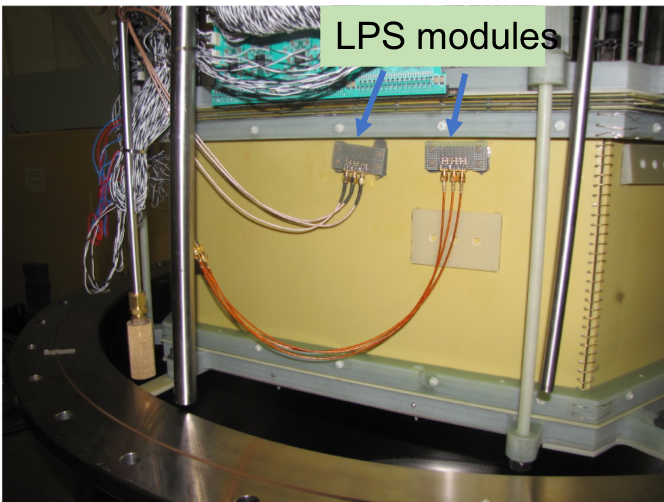
\includegraphics[width=0.6\linewidth]{LPS_miniCAPTAINlabeled.png} 
%\caption{Photo of the miniCAPTAIN TPC with two LPS modules glued on the outside to detect laser beam spot location via fluorescence of the TPC FR4 wall when illuminated by the laser beam.}
%\label{fig:miniCAPTAIN} 
%\end{figure}

\begin{dunefigure}[Laser positioning system modules in the miniCAPTAIN TPC]{fig:LPS_miniCAPTAINlabeled}
{Photograph of the mini\dword{captain} \dword{tpc} with two LPS modules glued on the outside to detect laser beam spot location via fluorescence of the \dword{tpc} FR4 wall when illuminated by the laser beam.}
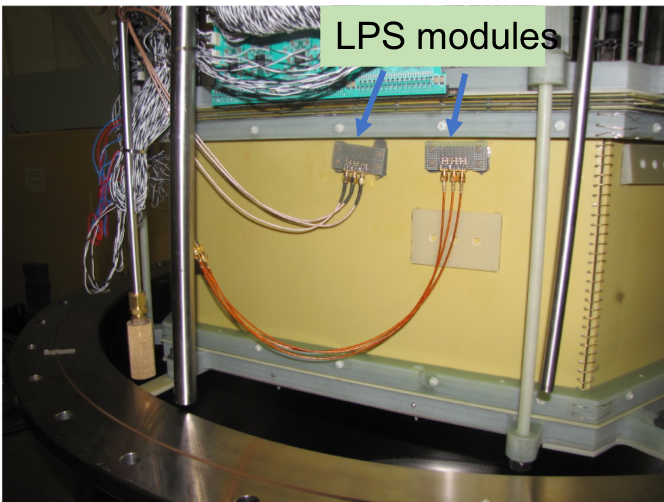
\includegraphics[width=0.6\linewidth]{LPS_miniCAPTAINlabeled} 
\end{dunefigure}

The LPS consists of groups of \num{9} pin diodes, operating in passive, photovoltaic mode. These are GaP diodes whose sensitivity range extends down to  \SI{200}{\nano\m} wavelength, so detecting \SI{266}{\nano\m} light is straightforward. Figure~\ref{fig:GaP_diode_room_temp} shows signals detected at room and cryogenic temperatures. The PIN diode was illuminated by the \SI{266}{\nano\m} light from the Nd:Yag
laser in the laboratory 
%(in the lab at University of Hawaii) 
set at lowest possible setting for minimal power. 

Pin diodes are placed at the bottom of the cryostat and receive light passing through the cathode and ground grids.
%gaps between the field cage profiles to minimize interference with the field cage. 
Drawings of one such group of pin diodes are shown in Figure~\ref{fig:GaP_assembly}. With the group of \num{9} photodiodes, not only can the beam be detected the beam but also its profile crudely characterized, giving a more precise location of the central beam pulse axis.


%\begin{figure}[htb!] 
%\begin{minipage}[b]{0.47\textwidth}
%\centering 
%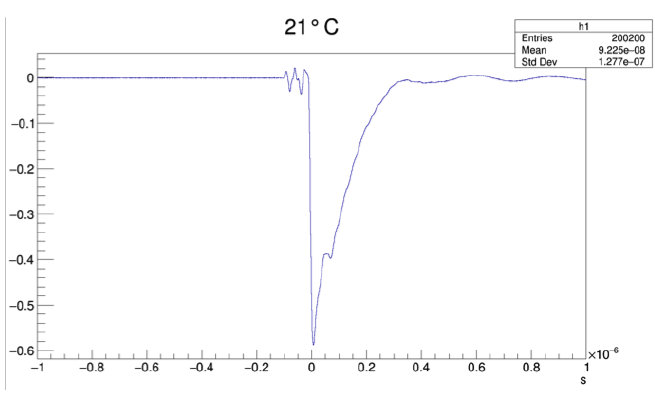
\includegraphics[width=0.95\linewidth]{GaP_diode_room_temp.png} 
%\caption{Signal from the GaP pin diode. The signal was a result of illumination of the PIN diode face with a 266\,nm laser at room temperature.}
%\label{fig:LPS1} 
%\end{figure}
%\end{minipage}
%\hfill
%\begin{minipage}[b]{0.47\textwidth}
%\begin{figure}[htb!] 
%\centering 
%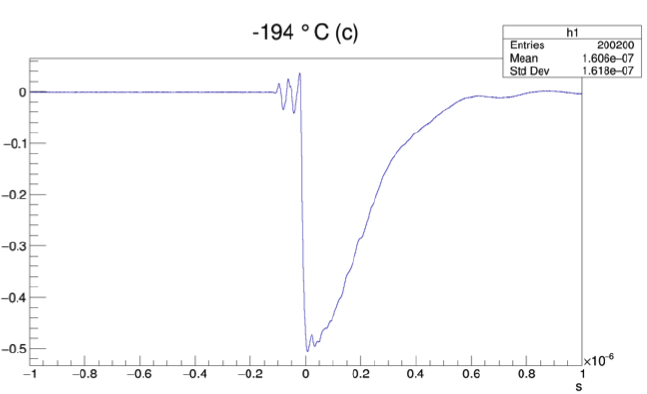
\includegraphics[width=0.95\linewidth]{GaP_diode_cryo_temp.png} 
%\caption{Signal from the GaP pin diode. The signal was result of illumination of the PIN diode face with a 266\,nm laser at cryogenic temperature.}
%\label{fig:LPS2} 
%\end{minipage}
%\hfill
%\end{figure} 


%\begin{figure}[htb!] 
%\begin{minipage}[b]{0.47\textwidth}
%\centering 
%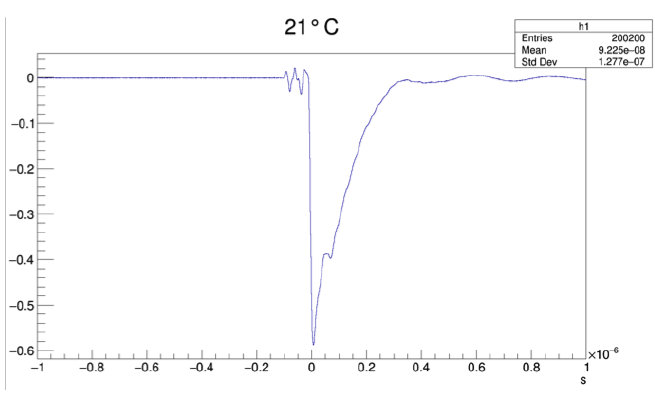
\includegraphics[width=1.0\linewidth]{GaP_diode_room_temp.png} 
%\caption{Signal from the GaP pin diode. The signal was a result of illumination of the PIN diode face with a 266\,nm laser at room temperature.}
%\label{fig:LPS1} 
%\end{minipage}
%\hfill
%\begin{minipage}[b]{0.47\textwidth}
%\centering 
%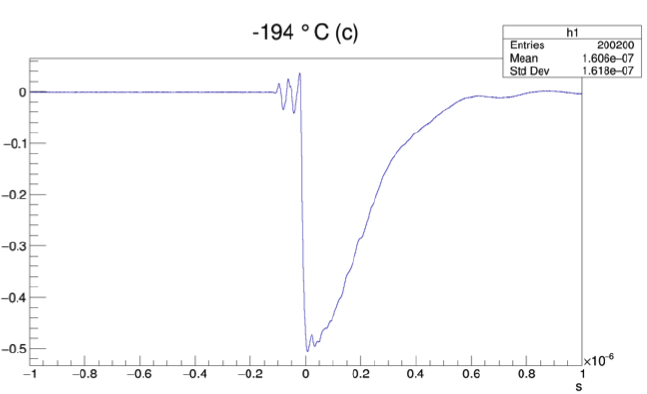
\includegraphics[width=1.0\linewidth]{GaP_diode_cryo_temp.png} 
%\caption{Signal from the GaP pin diode. The signal was result of illumination of the PIN diode face with a 266\,nm laser at cryogenic temperature.}
%\label{fig:LPS2} 
%\end{minipage}
%\hfill
%\end{figure} 


\begin{dunefigure}[Signal from the miniCAPTAIN laser positioning system at room and cryogenic temperatures]{fig:GaP_diode_room_temp}
{Signal from the miniCAPTAIN laser positioning system GaP pin diode. The signal was a result of illuminating the PIN diode face with a \SI{266}{\nano\m} laser at room (left) and cryogenic (right) temperatures.}
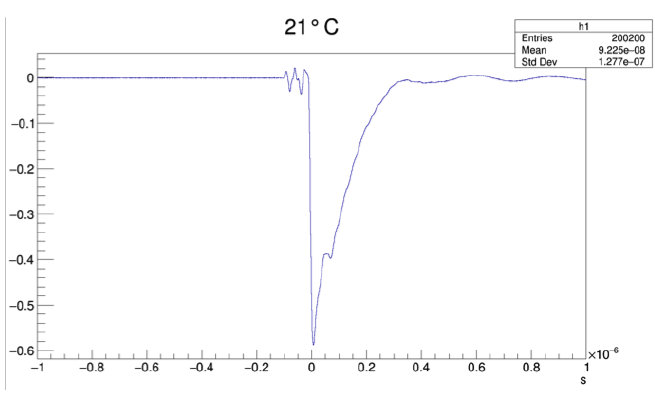
\includegraphics[width=0.47\linewidth]{GaP_diode_room_temp.png} 
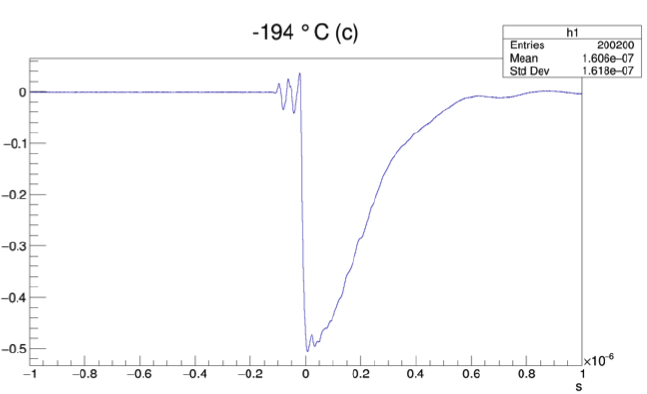
\includegraphics[width=0.47\linewidth]{GaP_diode_cryo_temp.png} 
\end{dunefigure}



\begin{dunefigure}[Cluster assembly of the miniCAPTAIN laser positioning system]{fig:GaP_assembly}
{(Left) LPS cluster mounted on the opposite wall from the laser periscope to detect and accurately determine the end point of the laser beam. (Right)
Profile of the LPS group mounted on the PCB. GaP diodes come with pins that use pairs of twisted wires to transport the signal.
}
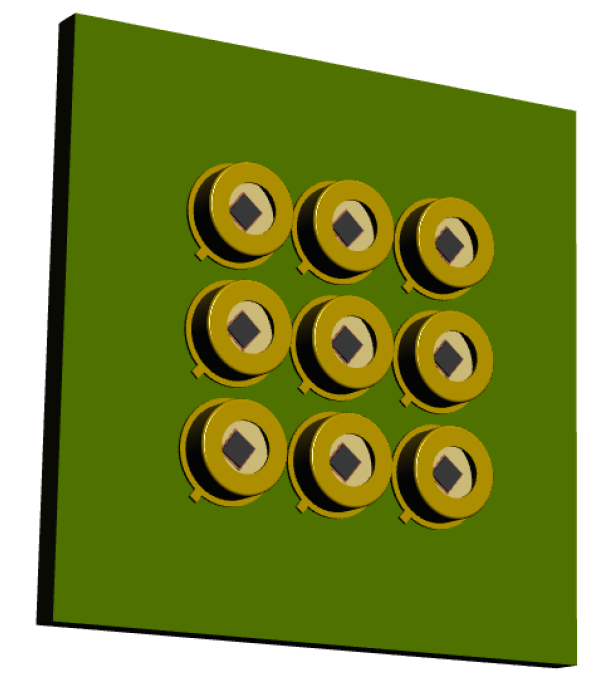
\includegraphics[width=0.47\linewidth]{GaP_assembly.png} 
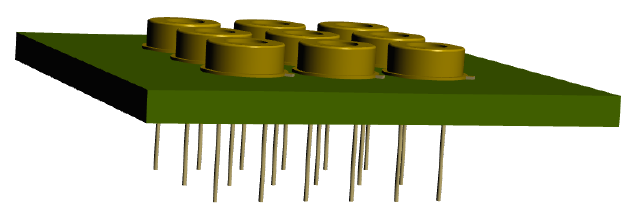
\includegraphics[width=0.47\linewidth]{GaP_assembly_profile.png} 
\end{dunefigure}


There will be one LPS pad per laser periscope. Laser always send the first pulse in the direction of the LPS before going into a calibration sequence. 
%The electronics used to collect signals from the LPS will be provided by \dword{cisc}.\todo{CISC doesn't provide electronics. SG emails Jelena to clarify this.}


\paragraph{Mirror-based beam positioning system:}

In addition to the pin-diode system, we will also have clusters of small mirrors that allow measuring the beam end position using its reflection.

Figure~\ref{fig:laser_mirror_positioning} shows a conceptual sketch with a cluster of 6 mirrors located close to each other but at different angles. When the beam hits one mirror, it will be reflected back into the \dword{tpc}, and the reflection angle unambiguously identifies which mirror was hit. Because the clusters of mirrors are small (a few cm), they fit inside the \dword{fc} profiles. With small mirrors, \SI{5}{\milli\m} in diameter, the required positioning precision would be met if these mirrors are placed at distances further than \SI{10}{\m}. The preferred location is, therefore, on the opposite \dword{fc} side wall. Because the top half of the \dword{fc} will be covered with \dword{pds} reflector panels, only lower half of the \dword{fc} profiles can be used. For redundancy, each laser periscope should have two associated mirror clusters, so the total number of clusters would be \num{32}. 

The simplest solution would be to have the reflecting surface made of polished aluminum, so the cluster could be a single block. Tests must be made of the actual reflectivity of the (oxidized) surface. An alternative would be small dielectric mirrors.

\begin{dunefigure}[Mirror-based laser beam positioning system]{fig:laser_mirror_positioning}
{View of the mirror cluster for the beam positioning system inserted in the \dword{fc} profiles~\cite{bib:yu2019a}.}
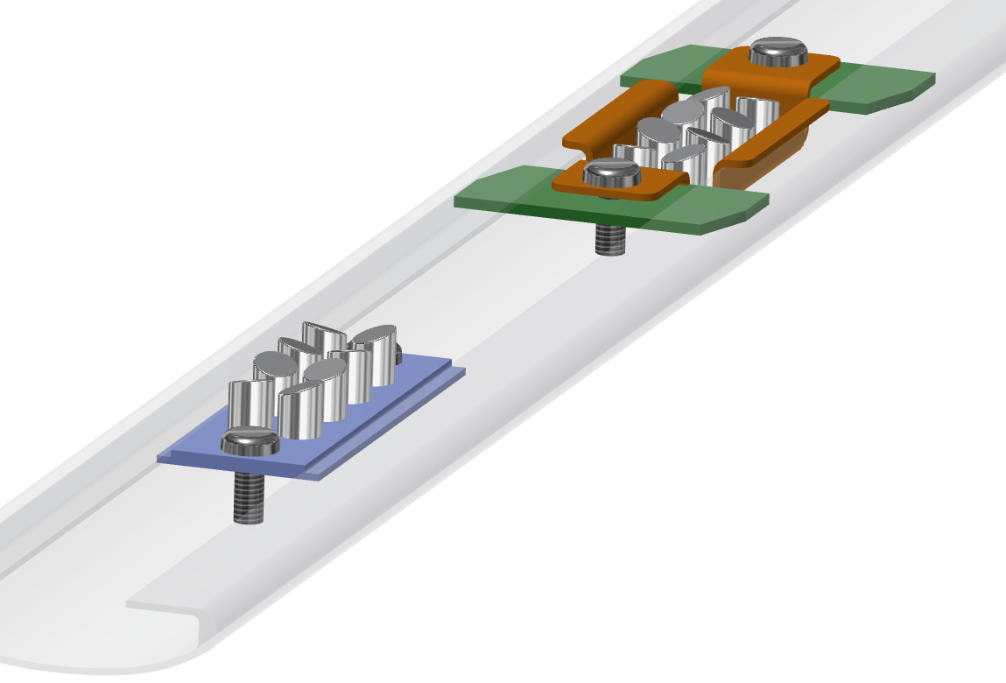
\includegraphics[width=0.7\linewidth]{laser_mirror_positioning.pdf}
\end{dunefigure}

\subsubsection{Development plan}
 The LPS assembly for reducing electronic noise and cross-talk must be further optimized, as must the size and shape of the cluster so that it would best collect the light coming through the cathode and ground grids.  Further, the system must be durable for extensive running under cryogenic conditions with  a large number of cool-downs to validate GaP for extended use in \dword{dune}. Finally, SiPMs are under consideration among other alternatives to GaP. While SiPMs require power, their sensitivity to single photons makes them desirable for low light signals and more accurate beam direction reconstruction. 
%KMTDRREADME:  What are noise rquirements and cross talk? 
%KMTDRREADME:  Does the LPS fail? Is it a big deal if it fails?
    















